% Created 2023-03-16 四 18:52
% Intended LaTeX compiler: xelatex
\documentclass[presentation]{beamer}
\usepackage{graphicx}
\usepackage{longtable}
\usepackage{wrapfig}
\usepackage{rotating}
\usepackage[normalem]{ulem}
\usepackage{amsmath}
\usepackage{amssymb}
\usepackage{capt-of}
\usepackage{hyperref}
\usepackage[UTF8,scheme=plain,fontset=fandol]{ctex}
\usetheme{default}
\author{Yong Zhou}
\date{\today}
\title{Visualization with Phoenix}
\hypersetup{
 pdfauthor={Yong Zhou},
 pdftitle={Visualization with Phoenix},
 pdfkeywords={},
 pdfsubject={},
 pdfcreator={Emacs 28.1 (Org mode 9.6.1)}, 
 pdflang={English}}
\begin{document}

\maketitle
\begin{frame}{Outline}
\tableofcontents
\end{frame}


\section{Visualization}
\label{sec:org9ea1783}
Online version: \url{https://ufan.site:444/phoenix/\#/megat}

\begin{itemize}
\item Load your own data and play with it
\begin{verbatim}
edm4hep2json tpcdrift_megat.root -o output.json -n 10 -l "TpcDriftHits,TpcSimHits"
\end{verbatim}
\end{itemize}
\begin{center}
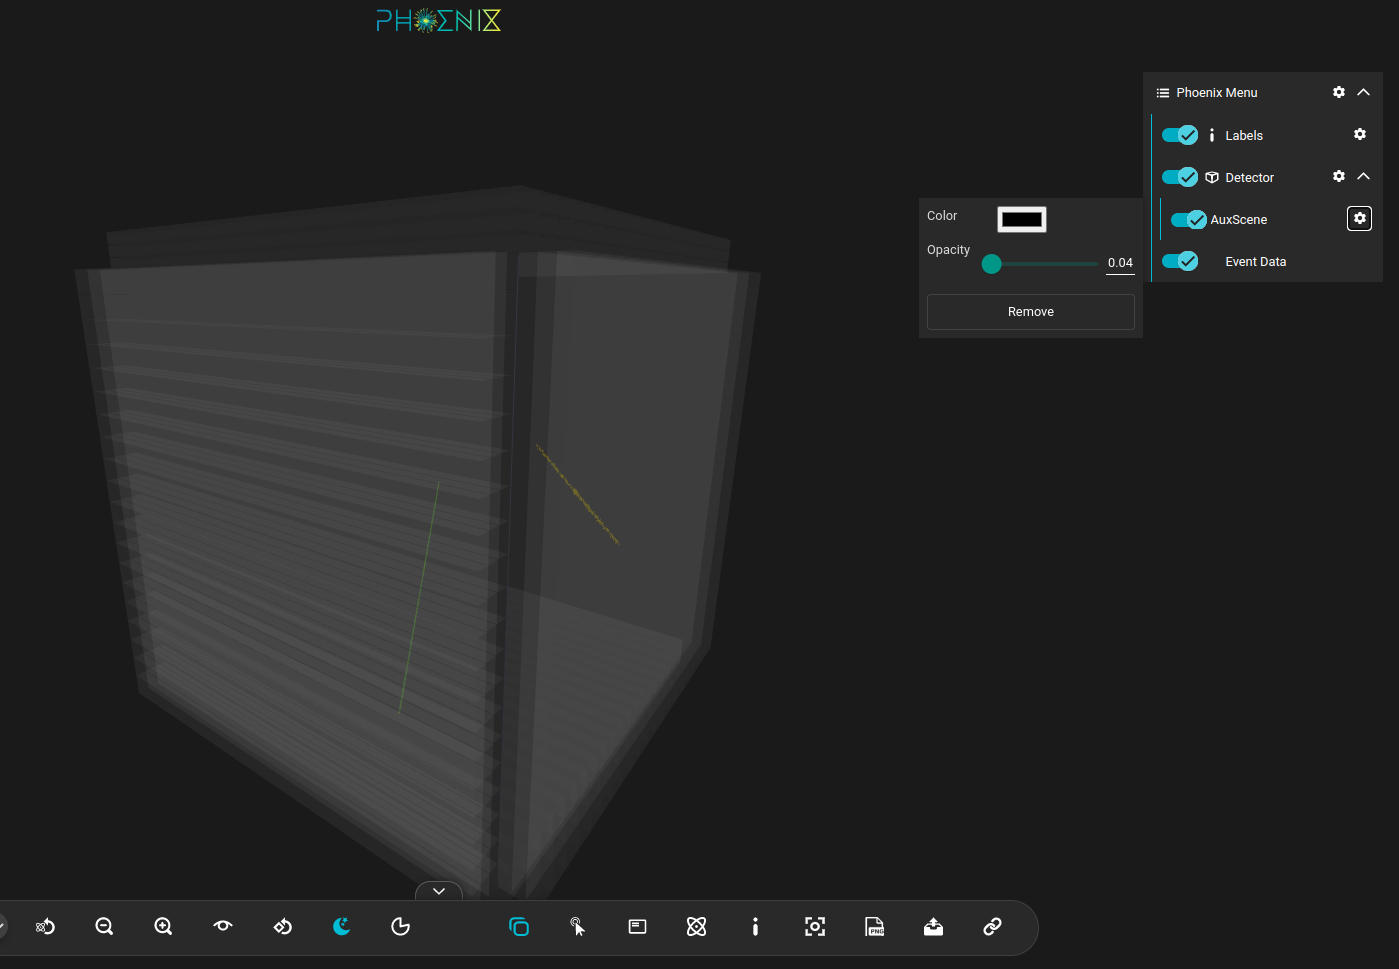
\includegraphics[width=.9\linewidth]{megat_online.png}
\end{center}
\end{document}